\documentclass[12pt,final,twoside]{report}
%%%%%%%%%%%%%%%%%%%%%%%%%%%%%%%%%%%%%%%%%%%%%%%%%%%%%%%%%%%%%
% Some credits:
% The template initially was created by Prof. Dr. Holger Karl/Uni Paderborn '2006
% and was expanded and updated by Dipl.-Inform. Stefan Heinrich/Uni Paderborn/Uni Hamburg since 2008.
% Suggestions for changes are always welcome.
%%%%%%%%%%%%%%%%%%%%%%%%%%%%%%%%%%%%%%%%%%%%%%%%%%%%%%%%%%%%%
% Meta information:
\newcommand{\trtitle}{Visual-Audio Integration for Object Recognition}
\newcommand{\trtype}{Master thesis} %{Diplomarbeit} %{Dissertation}
\newcommand{\trcourseofstudies}{Intelligent Adaptive Systems} %{Bioinformatik} 
\newcommand{\trauthor}{Weipeng He}
\newcommand{\trauthortitle}{} %{Dipl.-Inform.\ }
\newcommand{\tremail}{2he@informatik.uni-hamburg.de}
\newcommand{\trmatrikelnummer}{6411529}
\newcommand{\trstrasse}{Hagenbeckstra\ss e 60}
\newcommand{\trort}{22527 Hamburg}
\newcommand{\trgutachterA}{\href{mailto:zhang@informatik.uni-hamburg.de}{Prof. Dr. Jianwei Zhang}}
\newcommand{\trgutachterB}{\href{mailto:maeder@informatik.uni-hamburg.de}{Dr. Andreas M\"ader}}
%\newcommand{\trbetreuung}{\href{mailto:tbd@informatik.uni-hamburg.de}{Dipl.-Inform. To Be Defined}}
\newcommand{\trfach}{Technical Aspects of Multimodal Systems, TAMS}
\newcommand{\trdate}{30.03.2015}
\newcommand{\trkeywords}{Multimodal, HMM, Object Recognition}

%%%%%%%%%%%%%%%%%%%%%%%%%%%%%%%%%%%%%%%%%%%%%%%%%%%%%%%%%%%%%
% Languages:

% Falls die Ausarbeitung in Deutsch erfolgt:
% \usepackage[german]{babel}
% \usepackage[T1]{fontenc}
% \usepackage[latin1]{inputenc}
% \usepackage[latin9]{inputenc}                     
% \selectlanguage{german}

% If the thesis is written in English:
\usepackage[english]{babel}                         
\selectlanguage{english}

%%%%%%%%%%%%%%%%%%%%%%%%%%%%%%%%%%%%%%%%%%%%%%%%%%%%%%%%%%%%%
% Bind packages:
\usepackage{acronym}                    % Acronyms
\usepackage{algorithmic}                % Algorithms and Pseudocode
\usepackage{algorithm}                  % Algorithms and Pseudocode
\usepackage{amsfonts}                   % AMS Math Packet (Fonts)
\usepackage{amsmath}                    % AMS Math Packet
\usepackage{amssymb}                    % Additional mathematical symbols
\usepackage{amsthm}
\usepackage{booktabs}                   % Nicer tables
%\usepackage[font=small,labelfont=bf]{caption} % Numbered captions for figures
\usepackage{color}                      % Enables defining of colours via \definecolor
\definecolor{uhhRed}{RGB}{226,0,26}     % Official Uni Hamburg Red
\definecolor{uhhGrey}{RGB}{136,136,136} % Official Uni Hamburg Grey
\definecolor{uhhLightGrey}{RGB}{220, 220, 220}
\usepackage{fancybox}                   % Put equations in a frame
\usepackage{fancyhdr}                   % Packet for nicer headers
%\usepackage{fancyheadings}             % Nicer numbering of headlines
\usepackage[body={5.8in,9in}]{geometry} % Type area (size, margins...)

%\geometry{a4paper,outer=3.35cm}        % !!!Release version (Normal margins)
%\geometry{a4paper,outer=2.5cm}         % !!!Print version (Additional margin on the left for the binding)
%\geometry{a4paper}                     % !!!Proofread version (Additional margin on the right for corrections)
\geometry{a4paper,outer=3.15cm}         % !!!Draft version (Same margins on left and right)
%\geometry{paperheight=10.0in,paperwidth=6.4in,top=0.51in,left=0.3in}  % !!!Developer version (Minimal margins)

\usepackage{graphicx}                   % Inclusion of graphics
%\usepackage{latexsym}                  % Special symbols
\usepackage{longtable}                  % Allow tables over several parges
\usepackage{listings}                   % Nicer source code listings
\usepackage{multicol}                   % Content of a table over several columns
\usepackage{multirow}                   % Content of a table over several rows
\usepackage{rotating}                   % Alows to rotate text and objects
\usepackage{tabularx}                   % Tables with fixed width but variable rows
\usepackage{url,xspace,boxedminipage}   % Accurate display of URLs

%%%%%%%%%%%%%%%%%%%%%%%%%%%%%%%%%%%%%%%%%%%%%%%%%%%%%%%%%%%%%
% PDF Information und Definitions:
\author{\trauthor}

\ifx\pdftexversion\undefined
\usepackage{hyperref}
\else
\usepackage[colorlinks=false,           % link is colores (true) or has colored frame (false)
            linkcolor=uhhRed,           % case colorlinks=true: define color.
            urlcolor=uhhRed,
            citecolor=uhhRed,
            bookmarks,                  % Place bookmarks erstellen
            bookmarksopen=true,         % Bookmarks will be shown at start (true/false)
            pdfpagemode=UseOutlines,    
            bookmarksopenlevel=1,       % Define the depth of shown links
            bookmarksnumbered,          % Numbers of chapers in Bookmarks
            pdftitle={\trtitle},
            pdfsubject={\trtype},
            pdfkeywords={\trkeywords},
            pdfauthor={\trauthor},
            plainpages=false
            ]{hyperref}
\fi

%%%% added by hwp %%%%
\usepackage{subcaption}
\usepackage[symbol*]{footmisc}
\usepackage[capitalize]{cleveref}
\newcommand{\crefrangeconjunction}{--}

\ifx\pdftexversion\undefined
\else
\pdfoutput=1                            % Disable PDF-Output
\pdfimageresolution=1200
\pdfcompresslevel=2                     % 0 = no compression, 9 = strongest compression
\fi

%%%%%%%%%%%%%%%%%%%%%%%%%%%%%%%%%%%%%%%%%%%%%%%%%%%%%%%%%%%%%
% Configurationen:

\hyphenation{whe-ther}                  % Manually use: "\-" in a word: Staats\-ver\-trag

%\lstloadlanguages{C}                   % Set the default language for listings
\DeclareGraphicsExtensions{.pdf,.svg,.jpg,.png,.eps} % first try pdf, then eps, png and jpg
\graphicspath{{./fig/}}                 % Path to a folder where all pictures are located
\pagestyle{fancy}                       % Use nicer header and footer

% Redefine the environments for floating objects:
\setcounter{topnumber}{3}
\setcounter{bottomnumber}{2}
\setcounter{totalnumber}{4}
\renewcommand{\topfraction}{0.9}        %Standard: 0.7
\renewcommand{\bottomfraction}{0.5}     %Standard: 0.3
\renewcommand{\textfraction}{0.1}       %Standard: 0.2
\renewcommand{\floatpagefraction}{0.8}  %Standard: 0.5

% Tables with a nicer padding:
\renewcommand{\arraystretch}{1.2}

% Chapter and Sections will not be written in capitals
\renewcommand{\chaptermark}[1]{\markboth{\chaptername \ \thechapter.\ #1}{}}
\renewcommand{\sectionmark}[1]{\markright{\thesection.\ #1}}

%%%%%%%%%%%%%%%%%%%%%%%%%%%%
% Additional 'theorem' and 'definition' blocks:
\theoremstyle{plain}
\newtheorem{theorem}{Theorem}[chapter]
%\newtheorem{theorem}{Satz}[chapter]    % Wenn in Deutsch geschrieben wird.
\newtheorem{axiom}{Axiom}[chapter]     
%\newtheorem{axiom}{Fakt}[chapter]      % Wenn in Deutsch geschrieben wird.
%Usage:%\begin{axiom}[optional description]%Main part%\end{fakt}

\theoremstyle{definition}
\newtheorem{definition}{Definition}[chapter]

%Additional types of axioms:
\newtheorem{lemma}[axiom]{Lemma}
\newtheorem{observation}[axiom]{Observation}

%Additional types of definitions:
\theoremstyle{remark}
%\newtheorem{remark}[definition]{Bemerkung} % Wenn in Deutsch geschrieben wird.
\newtheorem{remark}[definition]{Remark} 

%%%%%%%%%%%%%%%%%%%%%%%%%%%%
% Provides TODOs within the margin:
\newcommand{\TODO}[1]{\marginpar{\emph{\small{{\bf TODO: } #1}}}}

%%%%%%%%%%%%%%%%%%%%%%%%%%%%
% Abbreviations and mathematical symbols
\newcommand{\modd}{\text{ mod }}
\newcommand{\RS}{\mathbb{R}}
\newcommand{\NS}{\mathbb{N}}
\newcommand{\ZS}{\mathbb{Z}}
\newcommand{\dnormal}{\mathit{N}}
\newcommand{\duniform}{\mathit{U}}

\newcommand{\erdos}{Erd\H{o}s}
\newcommand{\renyi}{-R\'{e}nyi}

\DeclareMathOperator*{\argmin}{arg\,min}
\DeclareMathOperator*{\argmax}{arg\,max}
% it is recommented to define complex terms as expression/newcommand and use the expression in the tex instead.

%%%%%%%%%%%%%%%%%%%%%%%%%%%%%%%%%%%%%%%%%%%%%%%%%%%%%%%%%%%%%
% Document:

\begin{document}

\pagenumbering{Roman}                   % Roman pagenumbering for lists and meta pages
\renewcommand{\headheight}{14.5pt}      % Size of headings

\thispagestyle{empty}
\fancyhead[LO,RE]{}                     % Define the header style for the meta pages

%%%%%%%%%%%%%%%%%%%%%%%%%%%%
% Cover sheet

\begin{titlepage}
%---Possibility 1:
    \begin{flushleft}
        
\includegraphics[width=85mm]{uhhLogoL.pdf}\\
    \end{flushleft}
%---Possibility 2:
%\includegraphics*[width=0.09\textwidth]{uhhIconR_}
%\parbox[c]{10cm}{
%    \begin{center}
%    Universit"at Hamburg --- MIN-Fakult"at\\
%    \trfachgruppe
%    \end{center}
%    }\hfill
%\includegraphics*[width=0.09\textwidth]{infIcon_}
%\vspace{0.2cm}
%---
    \rule{\textwidth}{0.4pt}
        \newline
        \vspace{2.0cm}
        \begin{center}
          \LARGE \textbf{\trtitle}
        \end{center}
    \vspace{2.0cm}
    \begin{center}
      \textbf{\trtype}\\
      %am Fachgebiet \trfach\\
      im Arbeitsbereich \trfach\\
      \trgutachterA\medskip\\
      Department Informatik\\
      MIN-Fakult\"at\\
      Universit\"at Hamburg \\[0.5cm]
      vorgelegt von \\
      \textbf{\trauthortitle\href{mailto:\tremail}{\trauthor}}\\
      am\\
      \trdate
    \end{center}
    \vspace{1cm}
    \begin{center}
    \begin{tabular}{ll}
    Gutachter: & \trgutachterA \\
                   & \trgutachterB \\
    %Betreuung: & \trbetreuung \\    	% Adviser are not allowed to demand getting credited, but are happy getting credited by the students initiative
    \end{tabular}
    \end{center}
    \vfill
    \begin{tabular}{l}
    \trauthor \\
    Matrikelnummer:  \trmatrikelnummer \\
    \trstrasse \\
    \trort
    \end{tabular}
    \newline
    \rule{\textwidth}{0.4pt}
    \newpage 
\end{titlepage}

    %backsite of cover sheet is empty!
\thispagestyle{empty}
\hspace{1cm}
\newpage

%%%%%%%%%%%%%%%%%%%%%%%%%%%%
% Abstract:
\section*{Abstract}\label{sec:abstract}
%\fancyhead[LE,RO]{\it Abstract}
%\addcontentsline{toc}{chapter}{\numberline{}Abstract}
Your English abstract here (mandatory if written in English and recommended otherwise).

\fancyhead[LE,RO]{\it Abstract}

\cleardoublepage

%%%%%%%%%%%%%%%%%%%%%%%%%%%%
% Lists:
\setcounter{tocdepth}{1}               % depth of the table of contents (for BSc and MSc Thesis 1 is recommented)
\fancyhead[LE,RO]{\it Contents}
\tableofcontents
\cleardoublepage
% List of Figures and List of tables are optional. -> Not needed in most theses.
\fancyhead[LE,RO]{\it List of Figures}
\listoffigures
\cleardoublepage
\fancyhead[LE,RO]{\it List of Tables}
\listoftables
\cleardoublepage
%\lstlistoflistings
%\cleardoublepage

\fancyhead[LE]{\it \leftmark}           % Define the header style for the text pages
\fancyhead[RO]{\it \rightmark}          % Define the header style for the text pages
\fancyhead[LO,RE]{}                     % Define the header style for the text pages

%%%%%%%%%%%%%%%%%%%%%%%%%%%%
% The content will be included here:
\pagenumbering{arabic}

\chapter{Introduction}
\section{Background}
\section{Objective}
\section{Contribution}
\section{Thesis Outline}

%\cleardoublepage
%\chapter{Background}
%In this chapter, three related fields regarding visual-audio object recognition will be reviewed. First, the traditional methods of object recognition based on visual information exclusively will be introduced. Then, the state-of-the-art in multimodal object recognition will be presented. Finally, the application of visual-audio integration in speech recognition will be explained.

\cleardoublepage
\chapter{Visual Object Recognition}
Visual object recognition has been extensively studied in the recent decade. Vision is very essential for both humans and artificial agents to recognize an object, since it provides the most direct and informational clue about the object. Numerous methods have been proposed for visual object recognition and they have been used in a variety of applications.

\begin{figure}[tbhp]
  \centering
  \begin{subfigure}[b]{.3\textwidth}
    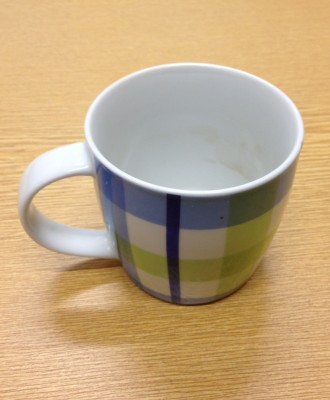
\includegraphics[width=\textwidth]{themug}
    \caption{Sam's coffee mug}
  \end{subfigure}
  ~
  \begin{subfigure}[b]{.3\textwidth}
    \centering
    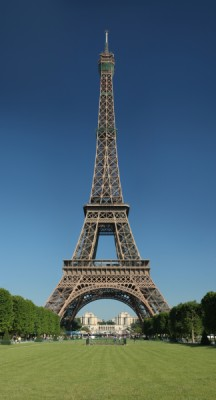
\includegraphics[width=.7\textwidth]{tour_eiffel}
    \caption{The Eiffel Tower\footnotemark}
  \end{subfigure}
  ~
  \begin{subfigure}[b]{.3\textwidth}
    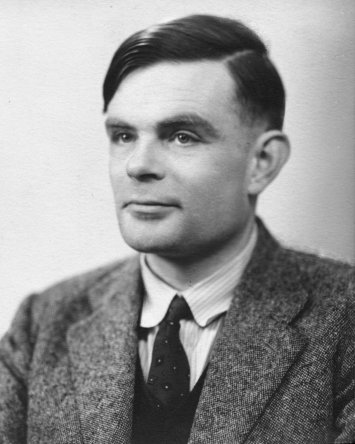
\includegraphics[width=\textwidth]{turing}
    \caption{Alan Turing}
  \end{subfigure}
  \caption{Examples of specific objects.}
  \label{fig:specific}
\end{figure}
\footnotetext{``Eiffel Tower'' by \href{http://commons.wikimedia.org/wiki/User:Benh}{Benh}. Licensed under \href{http://creativecommons.org/licenses/by-sa/3.0}{CC BY-SA 3.0}.}

Concerning object recognition, there are two types of tasks been studied: specific object recognition and object category recognition \cite{grauman_visual_2011}. The specific object recognition is the task of recognizing a particular object, place or person. Examples of this case are Sam's coffee mug, the Eiffel tower or Alan Turing as shown in \cref{fig:specific}. These objects (or person) have little variation in appearance and shape. 

\begin{figure}[tbhp]
  \centering
  \begin{subfigure}[b]{.45\textwidth}
    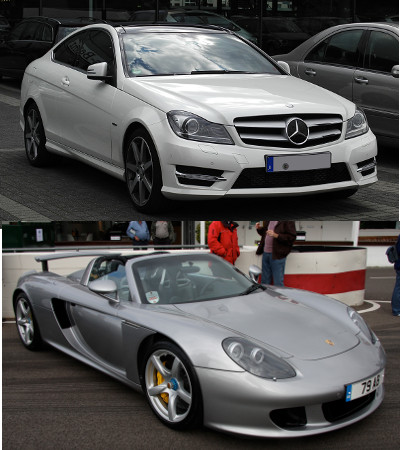
\includegraphics[width=.89\textwidth]{cars} % figure from public domain
    \caption{Cars\footnotemark}
  \end{subfigure}
  ~
  \begin{subfigure}[b]{.45\textwidth}
    \centering
    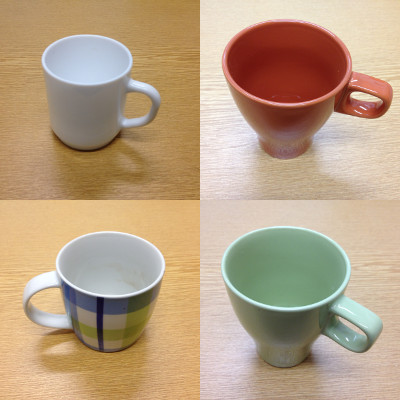
\includegraphics[width=\textwidth]{mugs}
    \caption{Coffee Mugs}
  \end{subfigure}
  \caption{Examples of generic objects categories.}
  \label{fig:generic}
\end{figure}
\footnotetext{The upper photo is ``Mercedes-Benz C 250'' by \href{http://commons.wikimedia.org/wiki/User:M_93}{M 93}. Licensed under \href{http://creativecommons.org/licenses/by-sa/3.0/de}{CC BY-SA 3.0 de}.
The lower photo is ``Porsche Carrera GT'' by \href{http://www.flickr.com/people/32659528@N00}{Brian Snelson}. Licensed under \href{http://creativecommons.org/licenses/by/2.0}{CC BY 2.0}}

Unlike the specific case, generic object category recognition cope with classifying an instance to a category, for example, telling a object is an instance of cars or coffee mugs (see \cref{fig:generic}). In this case, the objects belongs to the same category have the same conceptual meaning, but may vary in appearance and shape. A category can also be a function or an attribute of the object, like objects that can be sit on or soft objects.

As we have seen, these two types of tasks try to solve different problems. Therefore, different features and learning methods are required. Some of the approaches will be discussed in the rest of this section.

\section{Visual Specific Object Recognition}
One of the approaches which have achieved robust and efficient result in specific object recognition is proposed by Lowe \cite{lowe_object_1999}. His approach first extracts SIFT features from the image. Scale Invariant Feature Transform (SIFT)is a kind of local feature that is invariant to image translation, scaling, and rotation. Then, the extracted features are matched between train and test images. In the final step, the matched features are verified to confirm they are in a consistent geometric configuration. This approach has been widely used in robotic visual systems \cite{grauman_visual_2011}.

\section{Visual Object Category Recognition}
While specific object recognition can be solved as matching of local features, the task of object category recognition requires representations that capture the common characteristics of different instances in the same class. Example systems for object category recognition include the Viola-Jones face detector \cite{viola_rapid_2001}, bag-of-words model \cite{csurka_visual_2004} and HOG person detector \cite{dalal_histograms_2005}. 

The bag-of-words model \cite{csurka_visual_2004} for object category recognition is motivated by the bag-of-words model in text categorization. The visual image with a collection of local feature descriptors is analog to a document with a collection of words. In practice, a vocabulary of visual words is first constructed with clustering the feature descriptors from a number of images. Here, descriptors like SIFT or SURF can be used. Then, an image can be represented as a histogram of the vocabulary. After that, classifiers like support vector machine or Na\"ive Bayes can be used for categorization. This bag-of-words model achieved high and robust categorization accuracy.

Sivic et al. \cite{sivic_discovering_2005} used the bag-of-words model for unsupervised object categorization. Same as \cite{csurka_visual_2004}, given a collection of images, the feature of the images is first extracted as a bag of visual words. Then, generative models like Latent Semantic Analysis (pLSA) and Latent Dirichlet Allocation (LDA) are learned from the representation vectors. These models, which are successfully used for text analysis finding document topics, can also be used for finding the underlying common features of an object category. Since their learning method is unsupervised, it is applicable to a large unlabeled image set.

\cleardoublepage
\chapter{Visual Features}
\section{Scale-invariant Feature Transform}
\section{Bag of Visual Words Model}

\cleardoublepage
\chapter{Acoustic Features}
\section{Short Time Fourier Transform}
\section{Mel-frequency Cepstrum Coefficient}

\cleardoublepage
\chapter{Methods for Multimodal Object Recognition}
When thinking of how humans recognize objects, we use not only visual information, but also perceptions of other modalities, like auditory, haptic and olfactory perception. These extra perceptions provide complementary information. For example, a paper cup might have the same shape as a ceramic cup, and it is difficult to distinguish them only with vision. However, if we make some sound of them by knocking or touch them, we can use auditory or haptic information to tell the difference. This idea of multimodal object recognition is also applied to robotic systems.

\section{Multimodal pLSA Model}
Nakamura et al. \cite{nakamura_multimodal_2007} proposed an unsupervised object categorization method for robots based on visual, audio and haptic information. They used a multimodal pLSA model, which is extended from the pLSA model described in \cite{sivic_discovering_2005}, for the categorization.

In their experiment, a robot hand was used to grasp and shake the objects. During the interaction, visual, audio and haptic information were collected by a camera at the side, a microphone and pressure sensors on the robot finger. Afterwards, the data were processes separately as follows:
\begin{description}
  \item[Visual Information] \hfill \\
    Each image frame was represented using a bag-of-words model with scale and affine invariant salient region detector \cite{mikolajczyk_scale_2004} and SIFT descriptor \cite{lowe_distinctive_2004}. The visual vocabulary was generated by clustering the local descriptors in a collection of images into 600 clusters using k-means algorithm. The collection of images are 100 indoor images, which are independent of the objects in their experiment.
  \item[Audio Information] \hfill \\
    For each audio frame, a 13-dimensional MFCC feature was first calculated and then represented as a bag-of-words model with a vocabulary of 50 clusters. The vocabulary was generated with speech and noises.
  \item[Haptic Information] \hfill \\
    For each grasp of an object, a 2-dimensional feature vector was collected by the pressure sensors on the robot finger. Then, the feature vectors were vector quantized with 5 clusters, which was generated in advance.
\end{description}

They tested the unsupervised categorization on 40 objects in 8 categories. The objects were toys like stuffed toys, rattles, tambourines and balls. It was shown that their categorization result of using three modalities was identical to the categorization result of human subject. However, categorization using one modality alone did not work as well.

Furthermore, they also tested the performance of category and property inference of an unseen object. By using ``fold in'' heuristic \cite{hofmann_probabilistic_1999}, they correctly inferred the categories of all the objects in leave-one-out cross validation. For the property inference, their method can infer the auditory and haptic properties when given only the visual cue of the object.

\section{Behavior-Grounded Relational Learning}
Another multimodal object categorization approach is the behavior-grounded relational learning proposed by Sinapov and Stoytchev \cite{sinapov_object_2011}. Different from the aforementioned multimodal pLSA approach, they used different features and a supervised learning method.

They used an upper-torso humanoid robot to interact with the objects and collect proprioceptive and auditory information. The interactions included five exploratory behaviors, which are lift, shake, drop, crush and push. The proprioceptive data was recorded with 7 joint torque sensors and the auditory data was recorded by a microphone mounted on the robot head.

The method for extracting proprioceptive and auditory features were described in \cite{bergquist_interactive_2009} and \cite{sinapov_interactive_2009}, respectively. Since the interactions spanned over time, the data recorded were sequences of vectors. Here, a proprioceptive vector consisted of the joint torques, and a auditory vector was a Short Time Fourier Transform (STFT) of the raw audio recording. These vectors were further quantized using Self-organizing Map (SOM). Then, one modality of one behavior execution could be represented as a sequence of nominal values, that are the states in the SOM. Furthermore, the similarity between two different sequence can be calculated with Needleman-Wunch alignment algorithm \cite{needleman_general_1970}.

Based on the similarity of executions recordings, they constructed the relational features. The relational features of an object are the average similarities to a known object sets (for example the objects which are or are not plastic cups). The sets were the objects of the 6 categories, which are plastic cups, pop cans, metal objects, soft objects, empty bottles and objects with content. And, with 10 sensorimotor context (a behavior-modality combination), a object is represented by a $10 \times 2 \times 6 = 120$ dimensional vector.

Consequently, they applied discriminative methods, like Support Vector Machine, k-Nearest Neighbor and Decision Tree, for learning the object category. They evaluated these methods with Cohen's kappa coefficient \cite{cohen_coefficient_1960}. Their approach achieved kappa coefficient from 0.4 to .85 for the recognition.

\cleardoublepage
\chapter{Theories of Hidden Markov Model}
The hidden Markov models (HMM) are statistical models for sequence data, which have been well-known and widely used by researchers \cite{rabiner_tutorial_1989, rabiner_fundamentals_1993}. Theories of HMM are initially published by Baum and his colleagues \cite{baum_statistical_1966, baum_maximization_1970}. They have been successfully applied to a number of research fields, including speech processing \cite{baker_dragon_1975, rabiner_fundamentals_1993}, image processing \cite{chen_off-line_1994}, bioinformatics \cite{koski_hidden_2001}, finance \cite{bhar_hidden_2004}, etc.

In this chapter, we will first introduce the formal definition of the HMM and then present the algorithms for evaluating probability and estimating the model parameters.

\section{Definition of HMM} \label{sec:hmm}
A hidden Markov model describes a probability distribution of a stationary discrete-time stochastic process under certain assumptions. These assumptions include that there is an unobserved or hidden state associated with every observation at each time and the states transition meets the Markov property (i.e. Markov assumption). More precisely, for one observed sequence, $\mathbf{x}=(x_t, t \in \mathbb{N})$, and its associated state sequence, $\mathbf{q}=(q_t, t \in \mathbb{N})$, the following properties hold:

\begin{enumerate}
  \item The conditional distribution of present observation (at a certain time $t$) depends only upon the present hidden state:
  \begin{equation}
    P(x_t|q_1, \dots, q_t, x_1, \dots, x_{t-1}) = P(x_t|q_t),\quad t \in \mathbb{N} 
    \label{eq:ob_prob}
  \end{equation}
  \item (Markov property) The conditional probability distribution of future hidden state of the process depends only upon the present state:
  \begin{equation}
    P(q_{t+1}|q_1, \dots, q_t, x_1, \dots, x_t) = P(q_{t+1}|q_t),\quad t \in \mathbb{N}
    \label{eq:markov_prop}
  \end{equation}
\end{enumerate}

Here, the observation can be on a discrete space ($x_t \in \{v_1, v_2, \dots, v_K\}$) or a continuous space ($x_t \in \mathbb{R}^d$) and the state space is discrete ($q_t \in \{1, 2, \dots, N\}$, with $N$ being the number of states). Since our system is exclusively used on continuous data, for simplicity, we will only consider the continuous observation space. Gaussian mixture models (GMM) are usually used to describe such observation probability distribution. In this case, the model is called HMM-GMM.

Given the aforementioned assumptions, one HMM can be specified with the following parameters:
\[ \theta = (A, B, \pi) \]
such that
\begin{itemize}
  \item $A$ is the transition probability, $A = \{a_{ij}\}$, in which 
    \[ a_{ij} = P(q_{t+1} = j | q_t = i), \quad i,j \in \{1, \dots, N\} \]
  \item $B$ is the observation probability distribution, $B = \{b_j(x)\}$, in which
    \[ b_j(x) = P(x_t = x | q_t = j), \quad i,j \in \{1, \dots, N\} \]
  \item $\pi$ is the initial state distribution, $\pi = \{\pi_j\}$, in which
    \[ \pi_j = P(q_1 = j), \quad i,j \in \{1, \dots, N\} \]
\end{itemize}

As for HMM-GMM, each $b_j(x)$, more specifically, is a probability density function (pdf) of a GMM, namely
\[ b_j(x) = \sum_{k=1}^M c_{jk} \mathcal{N}(x, \mu_{jk}, \Sigma_{jk}) \]
where $c_{jk}$ is the mixture weight (coefficient), $\mu_{jk}$ is the mean and $\Sigma_{jk}$ is the covariance matrix, each of the $k$-th component in state $j$ and $\mathcal{N}$ is the pdf of the Gaussian distribution. 

With the formal definition of HMM, there are still three problems of interest to be solved, in order to use HMM for real-world applications. These problems are:
\begin{enumerate}
  \item Given a model $\theta=(A, B, \pi)$, and an observation sequence $\mathbf{x} = (x_1 x_2 \dots x_T)$, what is the probability of the model generating such sequence, namely $P(\mathbf{x}|\theta)$?
  \item Given a model $\theta$, and an observation sequence $\mathbf{x}$, what is the most likely hidden state sequence $\mathbf{q} = (q_1 q_2 \dots q_t)$, namely $\argmax_{\mathbf{q}}P(\mathbf{x}|\mathbf{q},\theta)$?
  \item Given an observation sequence $\mathbf{x}$ (or a set of observations $\{\mathbf{x}^{(i)}\}$), how do we estimate the parameters that maximize $P(\mathbf{x}|\theta)$ (or $\prod_{i} P(\mathbf{x}^{(i)}|\theta) $)?
\end{enumerate}

In the following section, we will show that the first and third problem can be solved using the forward/backward procedure and the Baum-Welch algorithm, respectively. The second problem can be solved using the Viterbi algorithm \cite{forney_viterbi_1973}. However, the second problem is not related to our system, so it will not be addressed.

\section{Probability Evaluation}
Given a model $\theta=(A, B, \pi)$, and an observation sequence $\mathbf{x} = (x_1 x_2 \dots x_T)$, we wish to calculate the probability, $P(\mathbf{x}|\theta)$. A na\"ive solution to this is enumerating all possible state sequences and applying law of total probability, that is
\begin{equation}
  P(\mathbf{x}|\theta) = \sum_{\text{all } \mathbf{q}} P(\mathbf{x}|\mathbf{q},\theta) P(\mathbf{q}|\theta) .
\end{equation}

For a fixed state sequence $\mathbf{q} = (q_1 q_2 \dots q_T)$, we can derive that
\begin{align}
  P(\mathbf{x}|\mathbf{q},\theta) &= P(x_1|q_1,\theta) P(x_2|q_1,q_2,x_1,\theta) \dots P(x_T|q_1,\dots,q_T,x_1,\dots,x_{T-1},\theta) \notag\\
  &= P(x_1|q_1, \theta) P(x_1|q_1, \theta) \dots P(x_T|q_T, \theta) \notag\\
  &= b_{q_1}(x_1) b_{q_2}(x_2) \dots b_{q_T}(x_T)
\end{align}
and its probability is
\begin{align}
  P(\mathbf{q}|\theta) &= P(q_1|\theta) P(q_2|q_1,\theta) P(q_3|q_1,q_2,\theta) \dots P(q_T|q_1,\dots,q_{T-1},\theta) \notag\\
  &= P(q_1|\theta) P(q_2|q_1,\theta) P(q_3|q_2,\theta) \dots P(q_T|q_{T-1},\theta)  \notag\\
  &= \pi_{q_1} a_{q_1q_2} \dots a_{q_{T-1}q_T} .
\end{align}
Thus we get 
\begin{equation}
  P(\mathbf{x}|\theta) = \sum_{q_1,q_2,\dots,q_T} \pi_{q_1} b_{q_1}(x_1) a_{q_1q_2} b_{q_2}(x_2) \dots a_{q_{T-1}q_T} b_{a_T}(x_T) .
  \label{eq:prob_brute}
\end{equation}

This is a direct solution, however, the number of possible state sequences is too large, which is $N^T$. Thus, the time efficiency would be $\Theta(T N^T)$ using big theta notation. That makes it impossible to calculate when $T$ is large, which is often the case. In the following part, we will present the forward procedure and the backward procedure, which are more efficient.

\subsection{The Forward Procedure}
One of the efficient solution is using the forward procedure. Consider the forward variable, $\alpha_t(i)$, which is the joint probability or the first $t$ observations and the state at time $t$, or defined as
\begin{equation}
  \alpha_t(i) = P(x_1,\dots,x_t,q_t=i|\theta) 
\end{equation}
it has the following properties:
\begin{enumerate}
  \item At initial time,
    \begin{equation}
      \alpha_1(i) = P(x_1,q_1=i|\theta) = \pi_i b_i(x_1), \qquad i \in \{1,\dots,N\} .
    \end{equation}
  \item The forward variable at $t \geq 2$ can be calculated via considering it is transitioned from all the possible previous states:
    \begin{align}
      \alpha_{t+1}(j) &= P(x_1,\dots,x_{t+1},q_{t+1}=j|\theta) \notag\\
      &= \sum_{i=1}^{N} P(x_1,\dots,x_{t+1},q_t=i,q_{t+1}=j|\theta) \notag\\
      &= \sum_{i=1}^{N} P(x_1,\dots,x_t,q_t=i|\theta) P(q_{t+1}=j|q_t=i,\theta) P(x_{t+1}|q_{t+1}=j,\theta) \notag\\
      &= \left[ \sum_{i=1}^{N} a_{ij} \alpha_t(i) \right] b_j(x_{t+1}), \qquad t \in \{1,\dots,T - 1\}, j \in \{1,\dots,N\} .
    \end{align}
  \item Take the sum of all the forward variables at time $t = T$, we get the desired calculation of the probability,
    \begin{equation}
      P(\mathbf{x}|\theta) = \sum_{i=1}^N P(\mathbf{x},q_T=i|\theta) = \sum_{i=1}^N \alpha_T(i) .
    \end{equation}
\end{enumerate}

By using the three properties, we can iteratively calculate all the $N$ forward variables from time $1$ to $T$. The time efficiency of the forward procedure is $\Theta(TN^2)$, which much faster than using the na\"ive solution (\cref{eq:prob_brute}).

\subsection{The Backward Procedure}
The backward procedure is an alternative solution to calculating the probability. Similar to the forward procedure, the backward procedure use the same idea of iterative calculation of variables based on previous steps, while the direction of iteration is backward, namely from $T$ to $1$. The backward variable is defined as
\begin{equation}
  \beta_t(i) = P(x_{t+1},\dots,x_T|q_t=i,\theta) .
\end{equation}

The following properties hold:
\begin{enumerate}
  \item At time $t = T$,
    \begin{equation}
      \beta_T(i) = 1, \qquad i \in \{1,\dots,N\} .
    \end{equation}
  \item The backward variable at $t \leq T - 1$ can be calculate inductively:
    \begin{align}
      \beta_i(t) &= \sum_{j=1}^{N} P(x_{t+1},\dots,x_T,q_{t+1}=j|q_t=i,\theta) \notag\\
      &= \sum_{j=1}^{N} P(q_{t+1}=j|q_t=i,\theta) P(x_{t+1}|q_{t+1}=j,\theta) P(x_{t+2},\dots,x_T|q_{t+1}=j,\theta) \notag\\
      &= \sum_{j=1}^{N} a_{ij} b_j(x_{t+1}) \beta_{t+1}(j) , \qquad t \in \{1,\dots,T - 1\}, j \in \{1,\dots,N\} .
    \end{align}
  \item The probability is
    \begin{equation}
      P(\mathbf{x}|\theta) = \sum_{i=1}^N P(\mathbf{x}|q_1=i,\theta) p(q_1=i|\theta) = \sum_{i=1}^N \beta_1(i) \pi_i .
    \end{equation}
\end{enumerate}

Same as the forward procedure, the time efficiency of the backward procedure is $\Theta(TN^2)$.

\section{Parameter Estimation}
Parameter estimation of a statistical model is the adjustment of the parameters such that the model can best match the observed or empirical data. It often plays a crucial role in systems. As for HMM, we are interested in knowing what are the parameters that maximize the probability of the observation (i.e. maximum likelihood estimates):
\begin{equation}
  \theta^* = \argmax_{\theta} P(\mathbf{x}|\theta) .
\end{equation}

Unlike simple models, such as Gaussian distributions, the parameters of which can be calculated directly, HMM depends on unobserved latent variables (i.e. hidden states), which make it difficult to estimate. One general solution for parameter estimation of models with latent variables is the expectation-maximization (EM) algorithm. The application of the EM algorithm for HMM is known as the Baum-Welch algorithm. We will shows these two algorithms in the following part.

\subsection{Expectation-maximization Algorithm}
The expectation-maximization algorithm is a method for finding the maximum likelihood estimates (MLE) of parameters of models with latent variables \cite{dempster_maximum_1977}. Its idea is reestimating parameters via an expectation step (E-step) and a maximization step (M-step), in which the reestimated parameters have greater likelihood, and repeating such process until the likelihood reaches a maximum.

More specifically, consider observed data $\mathbf{x}$, unobserved data (i.e. latent variables) $\mathbf{z}$ and a set of parameters $\theta$, the likelihood function is
\begin{equation}
  L(\theta;\mathbf{x}) = P(\mathbf{x}|\theta) = \sum_{\mathbf{z}} P(\mathbf{x},\mathbf{z}|\theta) .
\end{equation}
The goal is maximizing the likelihood function:
\begin{equation}
  \theta^* = \argmax_\theta L(\theta;\mathbf{x}).
\end{equation}

We introduce a function $Q(\theta|\theta')$, which is the conditional expectation of the log likelihood function with respect to the conditional distribution of $\mathbf{z}$ given $\mathbf{x}$ and $\theta'$:
\begin{equation}
  Q(\theta|\theta') = \text{E}_{\mathbf{z}|\mathbf{x},\theta'} \log P(\mathbf{x},\mathbf{z}|\theta) .
\end{equation}

A process of parameters reestimation consists of the following two steps:
\begin{description}
  \item[E-Step] Compute $Q(\theta|\theta^{(p)})$;
  \item[M-Step] Choose $\theta^{(p+1)}$ to be the value of $\theta$ that maximize $Q(\theta|\theta^{(p)})$.
\end{description}

After each process it is guarantied that $L(\theta^{(p+1)};\mathbf{x}) \geq L(\theta^{(p)};\mathbf{x})$. Therefore, if we start from an initial estimate $\theta^{(0)}$ and iteratively compute $\theta^{(1)},\theta^{(2)},\theta^{(3)},\dots$, we will get a sequence of estimates, which converges to a local maximum.

The increase of likelihood function can be proved as follows: for any $\mathbf{z}$, we have
\begin{equation}
  \log P(\mathbf{x}|\theta) = \log P(\mathbf{x},\mathbf{z}|\theta) - \log P(\mathbf{z}|\mathbf{x},\theta). 
\end{equation}
For both sides, if we multiply $P(\mathbf{z}|\mathbf{x},\theta')$ and sum over all $\mathbf{z}$, we get
\begin{align}
  \sum_{\mathbf{z}} P(\mathbf{z}|\mathbf{x},\theta') \log P(\mathbf{x}|\theta) 
    &= \sum_{\mathbf{z}} P(\mathbf{z}|\mathbf{x},\theta') \log P(\mathbf{x},\mathbf{z}|\theta)
    - \sum_{\mathbf{z}} P(\mathbf{z}|\mathbf{x},\theta') \log P(\mathbf{z}|\mathbf{x},\theta) \notag\\
  \log P(\mathbf{x}|\theta) &= Q(\theta|\theta') + H(\theta|\theta')
  \label{eq:loglph}.
\end{align}
Here, $H(\theta|\theta')$ is defined as
\begin{equation}
  H(\theta|\theta') = - \sum_{\mathbf{z}} P(\mathbf{z}|\mathbf{x},\theta') \log P(\mathbf{z}|\mathbf{x},\theta)
\end{equation}
From Gibbs' inequality we know that, for any $\theta$ and $\theta'$
\begin{equation}
  H(\theta|\theta') \geq H(\theta|\theta),
\end{equation}
with equality if and only if $\theta = \theta'$. Therefore, together with \cref{eq:loglph},
\begin{align}
  \log P(\mathbf{x}|\theta) - \log P(\mathbf{x}|\theta') &= Q(\theta|\theta') - Q(\theta'|\theta') + H(\theta|\theta') -  H(\theta|\theta) \notag\\
  & \geq Q(\theta|\theta') - Q(\theta'|\theta')
\end{align}

Since $\theta^{(p+1)}$ is a maximum of $Q(\theta|\theta^{(p)})$, $Q(\theta^{(p+1)}|\theta^{(p)}) - Q(\theta^{(p)}|\theta^{(p)}) \geq 0$. Therefore, $L(\theta^{(p+1)};\mathbf{x}) \geq L(\theta^{(p)};\mathbf{x})$.
  
It is important to note that although the EM algorithm converges to a maximum estimate, there is no guaranty that the estimate is a global maximum (thus not a MLE). The resulting estimate depends on the initial estimate. Therefore, additional heuristic methods should be chosen for application of the EM algorithm.

\subsection{Baum-Welch Algorithm}
We have shown that the EM algorithm can be used for parameter estimation for models with latent variables and HMMs are examples or such models. Thus, applying the EM algorithm to the HMM would result in a solution for the third problem we stated in \cref{sec:hmm}. This method is known as the Baum-Welch algorithm.

Before we proceed to derive the reestimation formulas, we first define variables $\gamma_t(i) = P(q_t=i|\mathbf{x},\theta)$ and $\xi_t(i,j) = P(q_t=i,q_{t+1}=j|\mathbf{x},\theta)$, which can be computed as follows:
\begin{align}
  \gamma_t(i) &= \frac{P(\mathbf{x},q_t=i|\theta)}{P(\mathbf{x}|\theta)} \notag\\
  &= \frac{\alpha_t(i)\beta_t(i)}{P(\mathbf{x}|\theta)} ,
  \label{eq:hmmgamma}
\end{align}
and
\begin{align}
  \xi_t(i,j) &= \frac{P(\mathbf{x},q_t=i,q_{t+1}=j|\theta)}{P(\mathbf{x}|\theta)} \notag\\
  &=  \frac{\alpha_t(i)a_{ij}b_j(x_{t+1})\beta_{t+1}(j)}{P(\mathbf{x}|\theta)} .
  \label{eq:hmmxi}
\end{align}

Now, we put the HMM into the frame of the EM algorithm.

\paragraph{E-step}
Consider parameters $\theta=(A,B,\pi)$ and $\theta'=(A',B',\pi')$ 
\footnote{We use `` $'$ '' to indicate parameters or variables from the previous estimate.}
, compute $Q(\theta|\theta')$:
\begin{align}
  Q(\theta|\theta') &= \sum_{\mathbf{q}} P(\mathbf{q}|\mathbf{x},\theta') \log P(\mathbf{x},\mathbf{q}|\theta) \notag\\
  &= \sum_{\mathbf{q}} \frac{P(\mathbf{x},\mathbf{q}|\theta')}{P(\mathbf{x}|\theta')} 
  (\log \pi_{q_1} + \sum_{t=1}^{T-1} \log a_{q_t q_{t+1}} + \sum_{t=1}^{T} \log b_{q_t}(x_t) ) \notag\\
  &= \frac{1}{P(\mathbf{x}|\theta')} (Q_\pi(\pi|\theta') + Q_A(A|\theta') + Q_B(B|\theta'))
  \label{eq:qhmmsep}
\end{align}
where
\begin{align}
  Q_\pi(\pi|\theta') &= \sum_{\mathbf{q}} P(\mathbf{x},\mathbf{q}|\theta') \log \pi_{q_1}  \notag\\
  &= \sum_{i=1}^{N} p(\mathbf{x},q_1=i|\theta') \log \pi_{i} \notag\\
  &= \sum_{i=1}^{N} \gamma'_1(i) \log \pi_{i},
\end{align}
\begin{align}
  Q_A(A|\theta') &= \sum_{\mathbf{q}} P(\mathbf{x},\mathbf{q}|\theta') \sum_{t=1}^{T-1} \log a_{q_t q_{t+1}} \notag\\
  &= \sum_{i=1}^{N} \sum_{j=1}^{N} \sum_{t=1}^{T-1} P(\mathbf{x},q_t=i,q_{t+1}=j|\theta') \log a_{ij} \notag\\
  &= \sum_{i=1}^{N} \sum_{j=1}^{N} (\sum_{t=1}^{T-1} \xi'_t(i, j)) \log a_{ij}
\end{align}
and
\begin{align}
  Q_B(B|\theta') &= \sum_{\mathbf{q}} P(\mathbf{x},\mathbf{q}|\theta') \sum_{t=1}^{T} \log b_{q_t}(x_t) \notag\\
  &= \sum_{i=1}^{N} \sum_{t=1}^{T} p(\mathbf{x},q_t=i|\theta') \log b_{i}(x_t) \notag\\
  &= \sum_{i=1}^{N} \sum_{t=1}^{T} \gamma'_t(i) \log b_{i}(x_t) .
  \label{eq:qhmmb}
\end{align}

\paragraph{M-step}
For fixed $\mathbf{x}$ and $\theta'$, to maximize $Q(\theta|\theta')$, we can see from \cref{eq:qhmmsep} that we only need to find parameters $\pi$, $A$ and $B$ that maximize $Q_\pi(\pi|\theta')$, $Q_A(A|\theta')$ and $Q_B(B|\theta')$, individually.

In order to be a valid distribution, the parameters subjects to the following constraints
\begin{align}
  \sum_{i=1}^{N} \pi_i &= 1  \\
  \sum_{j=1}^{N} a_{ij} &= 1 , \qquad \forall i 
\end{align}
and $b_i(x)$ is a valid probability density function of a GMM.

From Gibb's inequality, we know that the maximum of 
\begin{equation}
  \sum_{i=1}^N w_i \log y_i
\end{equation}
subject to $\sum_{i=1}^N y_i = 1$, is attained when
\begin{equation}
  y_i = \frac{w_i}{\sum_{j=1}^N w_j} .
\end{equation} 
Therefore, the reestimation of $\pi$ and $A$ are
\begin{equation}
  \pi_i = \frac{\gamma'_1(i)}{\sum_{j=1}^N \gamma'_1(j)} = \gamma'_1(i)
  \label{eq:hmmpi}
\end{equation} 
and
\begin{equation}
  a_{ij} = \frac{\sum_{t=1}^{T-1} \xi'_t(i,j)}{\sum_{k=1}^N \sum_{t=1}^{T-1} \xi'_t(i,k)} = \frac{\sum_{t=1}^{T-1} \xi'_t(i,j)}{\sum_{t=1}^{T-1} \gamma'_t(i)}
  \label{eq:hmma}
\end{equation} 

For the parameters $B$, from \cref{eq:qhmmb}, we can see that is it similar to reestiamting the parameters in a GMM, except that the terms are weighted with the expected occurrences of that state, $\sum_{t=1}^{T} \gamma'_t(i)$. And the result is as follows \cite{bilmes_gentle_1998}:
\begin{equation}
  c_{jk} = \frac{\sum_{t=1}^{T} \gamma'_t(j,k)}{\sum_{t=1}^{T} \sum_{l=1}^{M} \gamma'_t(j,l)},
  \label{eq:hmmc}
\end{equation}
\begin{equation}
  \mu_{jk} = \frac{\sum_{t=1}^{T} \gamma'_t(j,k) x_t}{\sum_{t=1}^{T} \gamma'_t(j,k)}
  \label{eq:hmmmu}
\end{equation}
and
\begin{equation}
  \Sigma_{jk} = \frac{\sum_{t=1}^{T} \gamma'_t(j,k) (x_t-\mu'_{jk})(x_t-\mu'_{jk})^T}{\sum_{t=1}^{T} \gamma'_t(j,k)}
  \label{eq:hmmsigma}
\end{equation}
where $\gamma'_t(j,k)$ is the probability of being state $j$ at time $t$ with the $k$-th mixture component (under the condition of the previous estimate $\theta'$):
\begin{equation}
  \gamma'_t(j,k) = \gamma'_t(j) \frac{c'_{jk} \mathcal{N}(x_t,\mu_{jk},\Sigma_{jk})} {b_j(x_t)} . \label{eq:hmmgamma2}
\end{equation}

To summarize, the reestimation of HMM parameters consists of the following steps:
\begin{enumerate}
  \item Compute $\alpha'_t(i)$ and $\beta'_t(i)$ using the forward and backward procedures;
  \item Compute $\gamma'_t(i)$, $\xi'_t(i,j)$ as well as $\gamma'_t(j,k)$ using \cref{eq:hmmgamma,eq:hmmxi,eq:hmmgamma2};
  \item Compute the new parameters $\pi_i$, $a_{ij}$, $c_{jk}$, $\mu_{jk}$ and $\Sigma_{jk}$ using \cref{eq:hmmpi,eq:hmma,eq:hmmc,eq:hmmmu,eq:hmmsigma}.
\end{enumerate}
And, by repeating these steps, we can get an estimate of the parameters which attain a local maximum of the likelihood function.

\cleardoublepage
\chapter{HMM Model for Bimodal Object Recognition}
\section{System Overview}
The models we use in our system for learning the categories are hidden Markov models with Gaussian Mixtures (HMM-GMM). For each category, we learn two models, one with the positive instances and the other with negative instances, using the Baum-Welch algorithm. The models by themselves cannot be used for classification, however, with some calculation we can get the posterior probability of an object being in the category and use this probability for classification:
\begin{equation}
  P(\mathbf{x}|\theta^+) = \frac{P(\mathbf{x}|\theta^+)P(\theta^+)}{P(\mathbf{x}|\theta^+)P(\theta^+) + P(\mathbf{x}|\theta^-)P(\theta^-)}
\end{equation}
where $\theta^+$ and $\theta^-$ are the positive and negative models, $\mathbf{x}$ is the observation, $P(\cdot|\theta^+)$ and $P(\cdot|\theta^-)$ are the probability density functions, and $P(\theta^+)$, $P(\theta^-)$ are the prior probabilities. Since we will use shifting classification threshold to calculate the receiver operating characteristic (ROC) curve afterwards, the prior probabilities can be assumed to be equal, and result in
\begin{equation}
  P(\mathbf{x}|\theta^+) = \frac{P(\mathbf{x}|\theta^+)}{P(\mathbf{x}|\theta^+) + P(\mathbf{x}|\theta^-)} .
\end{equation}
There are several parameters in HMM-GMM we can choose, which include the number of states, $n$, and the number of mixture components for each state, $k$. In our experiments, we tried the following four cases:
\begin{enumerate}
  \item $n = 1$ and $k = 1$;
  \item $n = 1$ and $k = 3$;
  \item $n = 3$ and $k = 3$;
  \item $n = 3$ and $k = 6$.
\end{enumerate}
The first two cases are degenerated forms of HMM-GMM, which are simply a Gaussian distribution and a Gaussian mixture model of three components, respectively. The parameters should be carefully chosen, for that small $n$ and $k$ may result in models that are too simple to learn the actual distribution, while large $n$ and $k$ may result in local optima or overfitting.

\section{Feature Extraction}
Given a video of interaction with an object, the visual and acoustic features are extracted as follows:
\subsection{Visual Feature}
First, the image frames from the raw video are taken at frame rate of 5 fps (frames per second). For each image frame, SIFT descriptors of all the key points are calculated. Then, all the descriptors are quantized using a codebook or a vocabulary of descriptors, which is prepared in advance. After that, the number of occurrences of the visual ``words'' are counted and represented as a histogram. At last, the histogram is normalized (sum of which equals 1) and we get the bag-of-words feature. Since the codebook we use contains 20 ``words'', the visual feature is a sequence of 20-dimensional vectors.

\subsection{Audio Feature}
The audio data are sampled at 8000 Hz. We first use shifting windows with window size of 1024 and shifting size of 1600 to get the audio frames, so that the rate of the audio frames is equal to that of the visual data. Then, we calculate the Mel-frequency cepstrum coefficients (MFCCs) with 32 filter banks. Among all the coefficients, from the second to the 17th are taken, resulting in a 16-dimensional vector. In this way, we get a sequence of MFCCs as the audio feature.


\section{Implementation Issues}
\subsection{Scaling}
\subsection{Diagonal Covariance Matrix}
\subsection{Initial Estimates}
\subsection{Parameter Selection}

\section{Methods for Bimodal Fusion}

\cleardoublepage
\chapter{Experiment and Results}
\section{Experiment Setup}

\section{Evaluation}
\section{Results}

\cleardoublepage
\chapter{Discussion and Conclusions}

%%%%%%%%%%%%%%%%%%%%%%%%%%%%
% Appendices:
% these are optional! For most Bachelor-theses and some Master-thesis none of them is needed. 
% Just comment them if not needed.
\cleardoublepage
\appendix
\fancyhead[LO,RE]{}                      % Define the header style for the appendixpages

\fancyhead[LE,RO]{\it Appendix}                %Adapt letter!
\chapter{app}

\cleardoublepage

% ... add as much appendices as you need (one can also add source code, for example)

%\fancyhead[LE]{\it \leftmark}
%\chapter{}
\fancyhead[LE,RO]{\it Bibliography}       % A bibliography never have a letter or numbering!
\bibliographystyle{plain}             % Style for presenting the literature
\addcontentsline{toc}{chapter}{Bibliography}% Add to the TOC
\bibliography{thesis}
\cleardoublepage

%%%%%%%%%%%%%%%%%%%%%%%%%%%%
% Formal page 1
\vspace{2cm}
\chapter*{Erkl\"arung der Urheberschaft}
\fancyhead[LE]{\it Erkl\"arung der Urheberschaft}
Ich versichere an Eides statt, dass ich die \trtype{} im Studiengang \trcourseofstudies{} selbstst\"andig verfasst und keine anderen als die angegebenen Hilfsmittel -- insbesondere keine im Quellenverzeichnis nicht benannten Internet-Quellen -- benutzt habe. Alle Stellen, die w\"ortlich oder sinngem\"a{\ss} aus Ver\"offentlichungen entnommen wurden, sind als solche kenntlich gemacht. Ich versichere weiterhin, dass ich die Arbeit vorher nicht in einem anderen Pr\"ufungsverfahren eingereicht habe und die eingereichte schriftliche Fassung der auf dem elektronischen Speichermedium entspricht.

%Ich versichere an Eides statt, dass ich die vorliegende \trtype{} selbstst\"andig und ohne unerlaubte Hilfe Dritter angefertigt habe. Alle Stellen, die inhaltlich oder w\"ortlich aus anderen Ver\"offentlichungen stammen, sind kenntlich gemacht. Diese Arbeit lag in gleicher oder \"ahnlicher Weise noch keiner Pr\"ufungsbeh\"orde vor und wurde bisher noch nicht ver\"offentlicht.

\vspace{4cm}
\noindent Ort, Datum \hfill Unterschrift

%The backcover is always empty
\newpage
\thispagestyle{empty}
\hspace{1cm}
\newpage

%%%%%%%%%%%%%%%%%%%%%%%%%%%%
% Formal page 2
\vspace{2cm}
\chapter*{Erkl\"arung zur Ver\"offentlichung}
\fancyhead[LE]{\it Erkl\"arung der Ver\"offentlichung}
Ich erkl\"are mein Einverst"andnis mit der Einstellung dieser \trtype{} in den Bestand der Bibliothek.

\vspace{4cm}
\noindent Ort, Datum \hfill Unterschrift

%The backcover is always empty
\newpage
\thispagestyle{empty}
\hspace{1cm}
\newpage

\end{document}

